\section{LEVEL 4 · Misleidingen en valkuilen}

\begin{missie}
Missie: laat je niet misleiden door cijfers, grafieken en slimme koppen. (LPD 1 – 3)
\end{missie}

\begin{doel}
\textbf{DOEL} \quad Na dit level kan je:

☐ valkuilen bij het \textbf{verzamelen} van data herkennen (steekproef, vraagstelling, opdrachtgever);

☐ \textbf{misleidende grafieken} herkennen en het misleidende effect uitleggen;

☐ misleidingen bij \textbf{numerieke} voorstellingen herkennen (gemiddelde of mediaan, \textbf{procent} of \textbf{procentpunt});

☐ procentuele veranderingen en procentpunten \textbf{berekenen} met ICT.
\end{doel}

\subsection*{Theorie 4.1 · Valkuilen bij het verzamelen van data}

\begin{theorie}
Tijdens het hele onderzoek moet je alert blijven. Bij het verzamelen van data let je op:

\begin{itemize}
\item \textbf{Representativiteit}: veralgemenen naar de hele populatie mag enkel bij een representatieve steekproef.
\item \textbf{Vraagstelling}: de manier waarop je een vraag formuleert, beïnvloedt het antwoord.
\item \textbf{Opdrachtgever}: wie betaalde het onderzoek? Is die gebaat bij een bepaald resultaat?
\end{itemize}
\end{theorie}

\begin{voorbeeld}
\textbf{Voorbeeld: vraagstelling.} Een gemeente wil een schermvrije speeltijd invoeren.

\textbf{Variant 1:} ‘Bent u voor of tegen een schermvrije speeltijd?’

\textbf{Variant 2:} ‘Schermvrije speeltijd zorgt voor meer beweging en betere vriendschappen. Bent u voor of tegen een schermvrije speeltijd?’

Bij variant 2 zal het percentage ‘voor’ groter zijn, omdat de voordelen al werden genoemd.

\textbf{Voorbeeld: opdrachtgever.} Uit een onderzoek bij 256 moeders blijkt dat 94 \% de nieuwe luiers aanraadt. Het onderzoek werd betaald door de luierfabrikant: de geloofwaardigheid is twijfelachtig.
\end{voorbeeld}

\subsection*{Theorie 4.2 · Misleidende grafieken}

\begin{theorie}
\begin{itemize}
\item \textbf{De as begint niet bij 0.} Heeft 0 een betekenis (bijvoorbeeld een score of percentage), dan moet de as bij 0 beginnen. Een afgeknotte as of scheurlijn laat verschillen veel groter lijken dan ze zijn.
\item Een \textbf{3D-cirkeldiagram}: wat op de voorgrond staat, lijkt groter dan wat op de achtergrond staat. Een 2D-cirkeldiagram heeft dit probleem niet.
\item Een \textbf{beelddiagram} (staven vervangen door figuren): vergroot je het figuurtje in alle richtingen, dan groeit de \emph{oppervlakte of het volume} veel sterker dan de waarde. Een staafdiagram geeft een eerlijker beeld.
\end{itemize}
\end{theorie}

\begin{center}
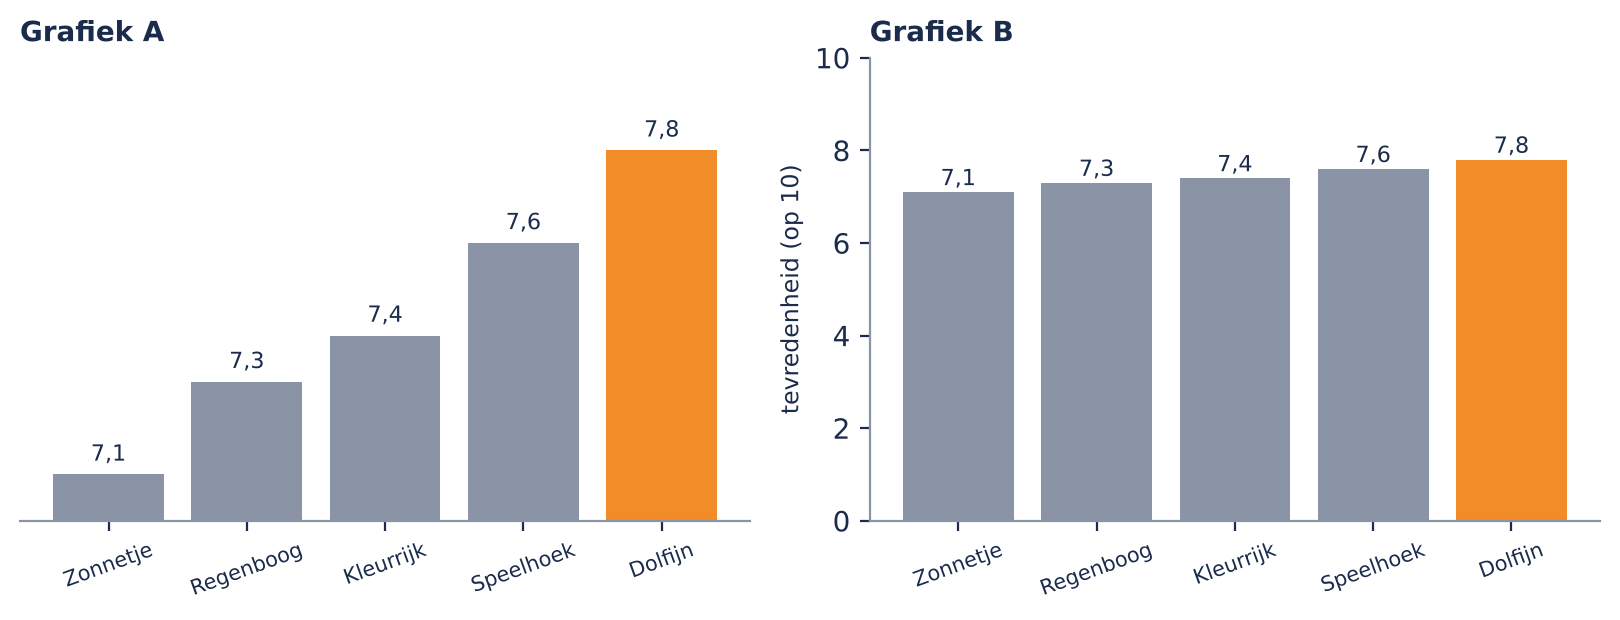
\includegraphics[width=0.95\textwidth]{figuren/d1_misleidend.png}
\end{center}

\begin{letop}
\textbf{LET OP} \quad Beide grafieken tonen dezelfde scores. In grafiek A lijkt de staaf van Dolfijn ongeveer 8 keer zo hoog als die van Zonnetje, terwijl de scores slechts 7,8 en 7,1 zijn. Grafiek B (as vanaf 0) is eerlijk.
\end{letop}

\subsection*{Theorie 4.3 · Misleidingen bij cijfers}

\begin{theorie}
\begin{itemize}
\item \textbf{Gemiddelde of mediaan?} Het gemiddelde is gevoelig voor uitschieters, de mediaan niet. Wie belang heeft, kiest de centrummaat die het best uitkomt.
\item \textbf{Procent of procentpunt?} Een verandering van een percentage kan je op twee manieren uitdrukken:
\begin{itemize}
\item absoluut in \textbf{procentpunt}: nieuw percentage min oud percentage;
\item relatief in \textbf{procent}: $\dfrac{\text{nieuw}-\text{oud}}{\text{oud}}\cdot 100\,\%$.
\end{itemize}
\end{itemize}
\end{theorie}

\begin{voorbeeld}
\textbf{Voorbeeld.} Het aandeel jongeren dat dagelijks sport stijgt van 40 \% naar 60 \%. Dat is een stijging van $60-40=20$ \textbf{procentpunt} en een stijging van $\dfrac{60-40}{40}=0{,}50=50\,\%$.

Een daling van 60 \% naar 30 \% is een daling van 30 procentpunt, of $\dfrac{30-60}{60}=-50\,\%$.
\end{voorbeeld}

\begin{ict}
\textbf{ICT-TIP} \quad In Excel typ je bijvoorbeeld =(60-40)/40 en geef je de cel de notatie ‘procent’. Maak je een grafiek in Excel of GeoGebra, controleer dan altijd of de verticale as bij 0 begint en of de assen een titel hebben.
\end{ict}

\subsection*{Aan de slag}

\subsubsection*{Oefening 4.1 \quad ★★☆ \quad Context: scores van kinderopvangen}

Bekijk de grafieken A en B in theorie 4.2 (tevredenheidsscores van vijf kinderopvangen).

\textbf{a)} Welke grafiek is misleidend? Welke misleiding zie je? \lijn

\textbf{b)} Wat is het misleidende gevolg voor de lezer? \lijn

\textbf{c)} Bereken met ICT: met hoeveel procent ligt de score van Dolfijn (7,8) hoger dan die van Zonnetje (7,1)? Rond af op 0,1 \%. \lijn

\textbf{d)} Weet je uit de grafieken hoeveel ouders werden bevraagd? Waarom is dat belangrijk? \lijn

\begin{oplossing}
\textbf{Oplossing 4.1} \quad a) Grafiek A: de verticale as begint niet bij 0 (en toont geen as). b) De verschillen lijken veel groter dan ze zijn: Dolfijn lijkt veel beter dan de rest. c) $\dfrac{7{,}8-7{,}1}{7{,}1}\approx 0{,}0986\approx 9{,}9\,\%$. d) Nee; zonder steekproefomvang kan je de betrouwbaarheid niet beoordelen.
\end{oplossing}

\subsubsection*{Oefening 4.2 \quad ★★☆ \quad Procent en procentpunt}

\textbf{a)} Kruis aan of vul aan: van 40 \% naar 60 \% is een toename van \_\_\_ procentpunt, dus van \_\_\_ procent. Van 60 \% naar 30 \% is een afname van \_\_\_ procentpunt, dus van \_\_\_ procent. \lijn

\textbf{b)} Vul aan: van 50 \% naar 70 \% is een toename van \_\_\_ procentpunt; van 35 \% naar 60 \% een toename van \_\_\_ procentpunt; van 80 \% naar 65,5 \% een afname van \_\_\_ procentpunt. \lijn

\textbf{c)} Bereken de relatieve verandering: van 44 \% naar 88 \% en van 88 \% naar 44 \%. \lijn

\textbf{d)} Een bank verhoogt de rente van 2 \% naar 2,5 \%. Druk de verhoging uit in procentpunt én in procent. \lijn

\begin{oplossing}
\textbf{Oplossing 4.2} \quad a) 20 procentpunt, 50 \%; 30 procentpunt, 50 \%. b) 20; 25; 14,5. c) $\frac{88-44}{44}=1=100\,\%$ toename; $\frac{44-88}{88}=-0{,}5=-50\,\%$, dus 50 \% afname. d) $2{,}5-2=0{,}5$ procentpunt; $\frac{2{,}5-2}{2}=0{,}25=25\,\%$.
\end{oplossing}

\subsubsection*{Oefening 4.3 \quad ★★★ \quad Context: dubbele korting}

Een winkel adverteert: ‘Jas van € 50: 60 \% korting, aan de kassa nog eens 20 \% extra!’ Een klant denkt dat de jas daardoor 80 \% korting heeft.

\textbf{a)} Bereken de prijs die de klant effectief betaalt. \lijn

\textbf{b)} Hoeveel procent korting is dat in totaal? Heeft de klant gelijk? \lijn

\begin{oplossing}
\textbf{Oplossing 4.3} \quad a) Na 60 \% korting: $50\cdot 0{,}40=20$ euro. Na nog 20 \%: $20\cdot 0{,}80=16$ euro. b) $\frac{50-16}{50}=0{,}68=68\,\%$ korting. De klant heeft geen gelijk: je mag de percentages niet optellen, want de tweede korting wordt op de al verlaagde prijs berekend.
\end{oplossing}

\subsubsection*{Oefening 4.4 \quad ★★☆ \quad Gemiddelde of mediaan?}

De maandlonen (bruto, in euro) van de negen medewerkers van een kinderopvang: 2\,400 – 2\,450 – 2\,500 – 2\,550 – 2\,600 – 2\,650 – 2\,700 – 2\,800 – 9\,000 (de laatste is de directeur).

\textbf{a)} Bereken met ICT het gemiddelde en de mediaan. \lijn

\textbf{b)} De directie wil tonen dat de lonen hoog zijn; de vakbond wil het tegendeel. Wie gebruikt welke centrummaat? \lijn

\textbf{c)} Welke centrummaat geeft het beste beeld van het typische loon? Verklaar. \lijn

\begin{oplossing}
\textbf{Oplossing 4.4} \quad a) $\overline{x}=\dfrac{29\,650}{9}\approx 3\,294{,}4$ euro; Med = 2\,600 euro. b) De directie gebruikt het gemiddelde (het is hoger), de vakbond de mediaan. c) De mediaan: het gemiddelde wordt door de uitschieter (9\,000 euro) omhooggetrokken; acht van de negen medewerkers verdienen minder dan 3\,294 euro.
\end{oplossing}

\subsubsection*{Oefening 4.5 \quad ★★☆ \quad Vraagstelling en opdrachtgever}

\textbf{a)} Welke formulering geeft waarschijnlijk meer ‘voor’-stemmen en waarom? (1) ‘Bent u voor of tegen een verbod op gsm’s tijdens de les?’ (2) ‘Gsm’s leiden vaak af en zorgen voor pestgedrag. Bent u voor of tegen een verbod op gsm’s tijdens de les?’ \lijn

\textbf{b)} ‘9 op 10 ouders vinden onze zoete ontbijtgranen gezond’, meldt de fabrikant, na een onderzoek dat de fabrikant zelf betaalde. Waarom blijf je kritisch? \lijn

\begin{oplossing}
\textbf{Oplossing 4.5} \quad a) Formulering 2: de voordelen van een verbod worden al genoemd (suggestieve vraag). b) De opdrachtgever heeft belang bij een gunstig resultaat; je weet niet hoe de steekproef en de vragen waren.
\end{oplossing}

\subsubsection*{Oefening 4.6 \quad ★★★ \quad Een bericht ontleden}

Een webshop schrijft: ‘Onze klanten zijn dol op de nieuwe babyfoon! 92 \% geeft 5 sterren!’ De scores komen van de beoordelingen die klanten vrijwillig online plaatsten.

\textbf{a)} Welke valkuil(en) zie je? Verklaar met begrippen uit deze bundel. \lijn

\textbf{b)} Welke gegevens zou je extra willen kennen om het bericht te beoordelen? \lijn

\begin{oplossing}
\textbf{Oplossing 4.6} \quad a) Vrijwillige respons (vooral tevreden of boze klanten schrijven een review) en de opdrachtgever is de verkoper: niet representatief voor alle klanten. b) Het aantal beoordelingen, het aantal verkochte exemplaren (responspercentage), hoe de beoordelingen werden verzameld en wie het onderzoek uitvoerde.
\end{oplossing}

\subsection*{Koppel · soort misleiding}

Koppel elke situatie (1 – 4) aan de misleiding (A – D).

\breedtes{58/42}
\begin{tabular}{ll}
\hline
Situatie & Misleiding \\
\hline
1. De verticale as van een staafdiagram begint bij 90. & A. suggestieve vraagstelling \\
2. ‘Wilt u ook het gezonde, natuurlijke product van ons?’ & B. gemiddelde wordt door uitschieters beïnvloed \\
3. ‘Het gemiddeld loon is 3\,300 euro’, maar de helft verdient minder dan 2\,600. & C. afgeknotte as \\
4. ‘De winst steeg met 20 \%’ terwijl het aandeel steeg van 50 \% naar 70 \%. & D. procent en procentpunt door elkaar gehaald \\
\hline
\end{tabular}

Mijn antwoord: 1 – \_\_\quad 2 – \_\_\quad 3 – \_\_\quad 4 – \_\_

\begin{oplossing}
\textbf{Oplossing Koppel} \quad 1 – C \quad 2 – A \quad 3 – B \quad 4 – D
\end{oplossing}

\subsection*{CHECK · Level 4}

\textbf{1.} (2 p) Noem twee manieren waarop een grafiek kan misleiden. \lijn

\textbf{2.} (2 p) Een percentage stijgt van 25 \% naar 30 \%. Geef de stijging in procentpunt en in procent. \lijn

\textbf{3.} (2 p) Waarom kan een gemiddelde misleidend zijn? \lijn

\textbf{4.} (2 p) Waarom moet je weten wie een onderzoek betaalde? \lijn

\begin{doel}
\textbf{Score:} \_\_\_ / 8 \quad ☐ behaald (vanaf 5 / 8) \quad ☐ nog even oefenen
\end{doel}

\begin{oplossing}
\textbf{Oplossing CHECK 4} \quad 1. De as begint niet bij 0; 3D-diagram of beelddiagram. 2. 5 procentpunt; $\frac{30-25}{25}=20\,\%$. 3. Uitschieters trekken het gemiddelde omhoog of omlaag, waardoor het niet typisch is; de mediaan niet. 4. De opdrachtgever kan baat hebben bij een bepaald resultaat, wat de geloofwaardigheid beïnvloedt.
\end{oplossing}
